Intro: The solution will be integrated into the existing AccessMap infrastructure.
(Caspi writes)

\jm{Notes from conversation with Harniss:
Emphasize iteration
Blow smoke about the algorithms
}
\jm{Notes from megan on call: +"Development Activities in appropriate enviroment"
++describe the enviroments that you are testing your "something"
++enviorment differs based on circumstance
++describe to the reviewer}

\subsection{State of the art for related products (mankoff\&caspi-relatedwork.tex)}
\jm{brandon's text. Write a similar intro paragraph: Tactile maps have a long history that predates 3D printing as a
commercially available technology. Embossers and microcapsule
paper can be used to automatically create maps from computergenerated images [23]. However, these techniques provide only
two layers of depth and require expensive equipment. Braille
embossers start at \$1800 and can range up to \$80,000 for highspeed machines [2]. Microcapsule, or swell paper, printers can be
had for \$1350 and also require specialized paper that costs more
than a \$1 per sheet [3]. Another production method, vacuum
forming, offers a wider range of possible tactile features.}

\ac{
Also not my text:

Mobility and orientation are  among the greatest challenges for visually impaired people.  One reason that explains these issues is that visually impaired users in general usually exchange or are given verbal descriptions of itineraries, which may help them to find their way, but do not provide them with  any  clue  about the  spatial  layout  of  the targeted  environment. GPS-based  systems,  although  facilitating  navigation,  raise  the  same  issue.  Sighted  people  usually acquire information about a spatial environment through visual perception or by using geographical maps.  However,  maps  are  essentially  visual  and  thus  inherently  inaccessible  for visually  impaired people.  And  weak access to  maps has drastic  consequences  on mobility  and  education, but  more generally on personal and professional life, and can lead to social exclusion (Passini & Proulx, 1988).  Beyond  orientation  and  mobility  purposes,  maps  are  very  useful  tools  to  explore  and  analyze geographical  data  and  to  acquire  general  knowledge  about  many  subjects  such  as  demography, geopolitics,  history,  etc. They  are  also often  used in  the classroom  for this  purpose. As  stated  by O’Modhrain  et  al.  (2015),  “there  is  an  immediate  need  for  research  and  development  of  new technologies to provide non-visual access to graphical material. While the importance of this access is  obvious  in  many  educational,  vocational,  and  social  contexts  for  visually  impaired  people,  the diversity of  the user group,  range  of available technologies, and  breadth  of tasks to  be  supported complicate the research and development process”.  In specialized educational centers for visually  impaired people,  tactile  maps are  commonly used  to give visually impaired students access to geographical representations. However, these materials are rarely used or available outside  of  school, because their  production  is a  costly and time-consuming process (Rice, Jacobson, Golledge, & Jones, 2005). To create a tactile map, one of the most common methods is to print it on a special paper, called “swell paper” (synonyms are “microcapsule paper” or “heat sensitive  paper”), which contains microcapsules  of alcohol  in  its coating.  When the  paper  is heated, the microcapsules expand and create relief over black lines (Figure 1.a). The resulting maps, called raised-line maps, can be perceived by touch. But they are also visual maps, making it possible to  share  information  between  blind  and  (partially)  sighted  people.  Raised-line  maps  are  usually prepared with a computer, which makes it possible to print and fuse several copies of the same map.  Another techniques, called vacuum-forming or thermoforming, consists in placing a sheet of plastic over a  master made of a variety of textured materials.  When it is heated in a vacuum, the sheet is permanently  deformed  according  to  the  master.  Hand-crafted  techniques  can  also  be  used  to produce maps and  other  graphics.  For example,  for orientation and mobility lessons,  teachers  and students construct itineraries or local maps, by progressively placing magnets over a magnetic board (Figure  1.b).  Students are  sometimes asked  to replicate  the  construction, so  that the  teacher can check  that  the  itinerary  has  been  memorized.  Small-scale  models  made  out  of  wood  also  exist, alongside  graphics  made  out  of  paper,  cardboard,  ropes,  etc.  (see  Figure  1.c).  Edman  (1992) presented a comprehensive summary of production techniques for accessible maps. 
   
   
   Although  tactile  maps  are  efficient  for  acquisition  of  spatial  knowledge,  they  present  several limitations  and  issues.  As  stated  by  Rice  et  al.  (2005)  the  production  of  tactile  maps  is  time consuming and expensive. In addition, tactile maps must be produced by a tactile graphics specialist who knows how to present information so that it can be perceived by touch (Tatham, 1991). Other critiques  concern  the  number  of  elements  that  can  be  displayed  and  the  accuracy  of  the  map content.  Indeed,  because  of  the  perceptual  limits  of  the  tactile  modality,  less  details  can  be represented on a tactile map  than  on  a visual map. Furthermore, once  a tactile  map is printed,  its content is static and cannot be adapted dynamically. Tactile maps are then quickly getting outdated (Yatani,  Banovic, &  Truong,  2012).  In  addition,  the  use  of  braille  labels  is  an  issue.  Only  a  small percentage  of  visually  impaired  people  read  braille  (National  Federation of  the Blind,  2009);  and braille is not so convenient when compared to printed text. Text on visual maps can be written with different font sizes and styles. It can be rotated to fit in open spaces. Upper and lower cases, as well as color, can be used to highlight important  items.  In  contrast,  braille  lacks all of these possibilities and needs a lot of  space  because it is  fixed  in  size, inter-cell spacing and orientation (A. F. Tatham, 1991). Due to the lack of space, braille abbreviations are commonly used on tactile maps, which are then explained in a legend accompanying the map. Because the reader must frequently move hands between  the  map and  the  legend, it  disrupts the  reading process  (Hinton,  1993). Finally,  because they  are  not  interactive,  tactile  maps  cannot  provide  advanced  functionalities  such  as  panning, zooming, annotating, computing itineraries or distances, and using filters to facilitate the exploration.
}

The greatest challenge in mobility and orientation for visually impaired people is to understand the spatial layout of the targeted environment. 
Although  tactile  maps  have proven comparatively efficient  for  acquisition  of  spatial  knowledge,  they  present  several limitations  and  issues.

With the advent of consumer-grade fabrication technologies, 3D printed and other custom fabricated maps have been receiving increasing attention. For example, it is now possible to requisition a custom, laser-cut topographical map on ETSY \cite{etsy} or purchase custom 3D printed topographic models through companies such as Sightline \url{sightlinemaps.com} or PrintMyRoute \url{www.printmyroute.xyz}. However, these services do not include features intended to support Blind or Blind/Deaf users, and do not support activities such as route finding and landmark identification as a result. 

The accessibility community has added its own spin to these technologies. For example TouchMapper \url{touch-mapper.org} is a free service that will create a tactile map using embossing or 3D printing and help connect you to existing online printing services or print it yourself.  This service focues on showing streets, and can be customized for size, inclusion of buildings and other features. However it too does not include route finding or landmark identification. 

From a research perspective, one open problem is combining tactile maps and smartphones. By embedding capacitive touch sensing capabilities in tactile maps, it is possible to provide audio feedback about the region someone is touching \cite{taylor2016customizable, rusu2010semantic,gotzelmann2016lucentmaps}. 

Another open question is which cartographic features should be highlighted in tactile maps \cite{haberling2008proposed}. Although some work has explored this design space, it did not focus on the needs of Deaf-Blind individuals, and no computational model that takes these variables into account exists.

Finally, questions remain about the ability to of tactile maps to support route finding (as opposed to orientation). For example, Gual \textit{et al.} found that standard 3D printed maps can improve memorization in route finding, but could not be used autonomously without collaborator support \cite{gual2012visual}. However, they did not explore a wide range of tactile variables to support interpretation. 

To summarize, tactile maps are not new to the cartographic record \cite{xx}. Their value in facilitating orientation and navigation for the low vision and blind communities has been well established \cite{XXX}. However, their scope and availability has been greatly limited in the past by high production costs and limited interest from fields traditionally invested in map making and design.  3D printing has significantly reduced the costs of producing such maps, but to our knowledge no existing product has enhanced 3D printed maps with optimization and customization, making our product and important addition to this space. 



\subsection{Extending the AccessMap interface to 3D printed map generation (Caspi-accessmap.tex)}
%jen: repeats words in the bcakground section Tactile maps are not new to the cartographic record. Their value in facilitating orientation and navigation for the low vision and blind communities has been well established. However, their scope and availability has been greatly limited in the past by high production costs and limited interest from fields traditionally invested in map making and design. 

% same These maps have been designed as tools that enhance spatial understanding for people within a large range of visual capacities.  They abstract nonvisual cues from the pedestrian environment and consider circumstances that influence a full spectrum of experience. 

\subsubsection{Background and State of the Art}

\begin{comment}
I believe this is used somewhere else. Need to pull in.

Independent navigation is essential for autonomy and community participation in urban centers. 
Navigation solutions for both sighted and blind individuals fall into two important categories -- turn by turn directions, and maps. 
A common solution for Blind navigators is GPS programs that provide turn by turn directions. We tested the three blindness-aware GPS navigation mobile apps recommended by the American Foundation for the Blind: "Nearby Explorer", "The Seeing Eye GPS App", and "BlindSquare", and none offered a simultaneously sparse and informative solutions when used in conjunction with a portable Braille reader \cite{AFBBlindnessNavApps}, often because it is difficult to consume a lot of information portably with Braille readers on the go, and not all the information was equally relevant. 

\end{comment}


\subsubsection{Previous Development}
\label{sec:prev-devel-access}
The Taskar Center has two other relevant projects aiming to improve access to mobility and transportation for individuals with disabilities. The Taskar Center's overarching goal is 
to develop seamless regular-commute transportation customized assistance system that integrates multiple sources of current and critically relevant travel information.

This project build on AccessMaps, which itself depends on data from OpenSidewalks. As we will show, \jm{key points for extending accessmaps}




AccessMaps is \jm{Anat fill in introduction}.
Figure~\ref{fig:accessmap} shows the current version of the system in use. 

\begin{figure}
    \centering
    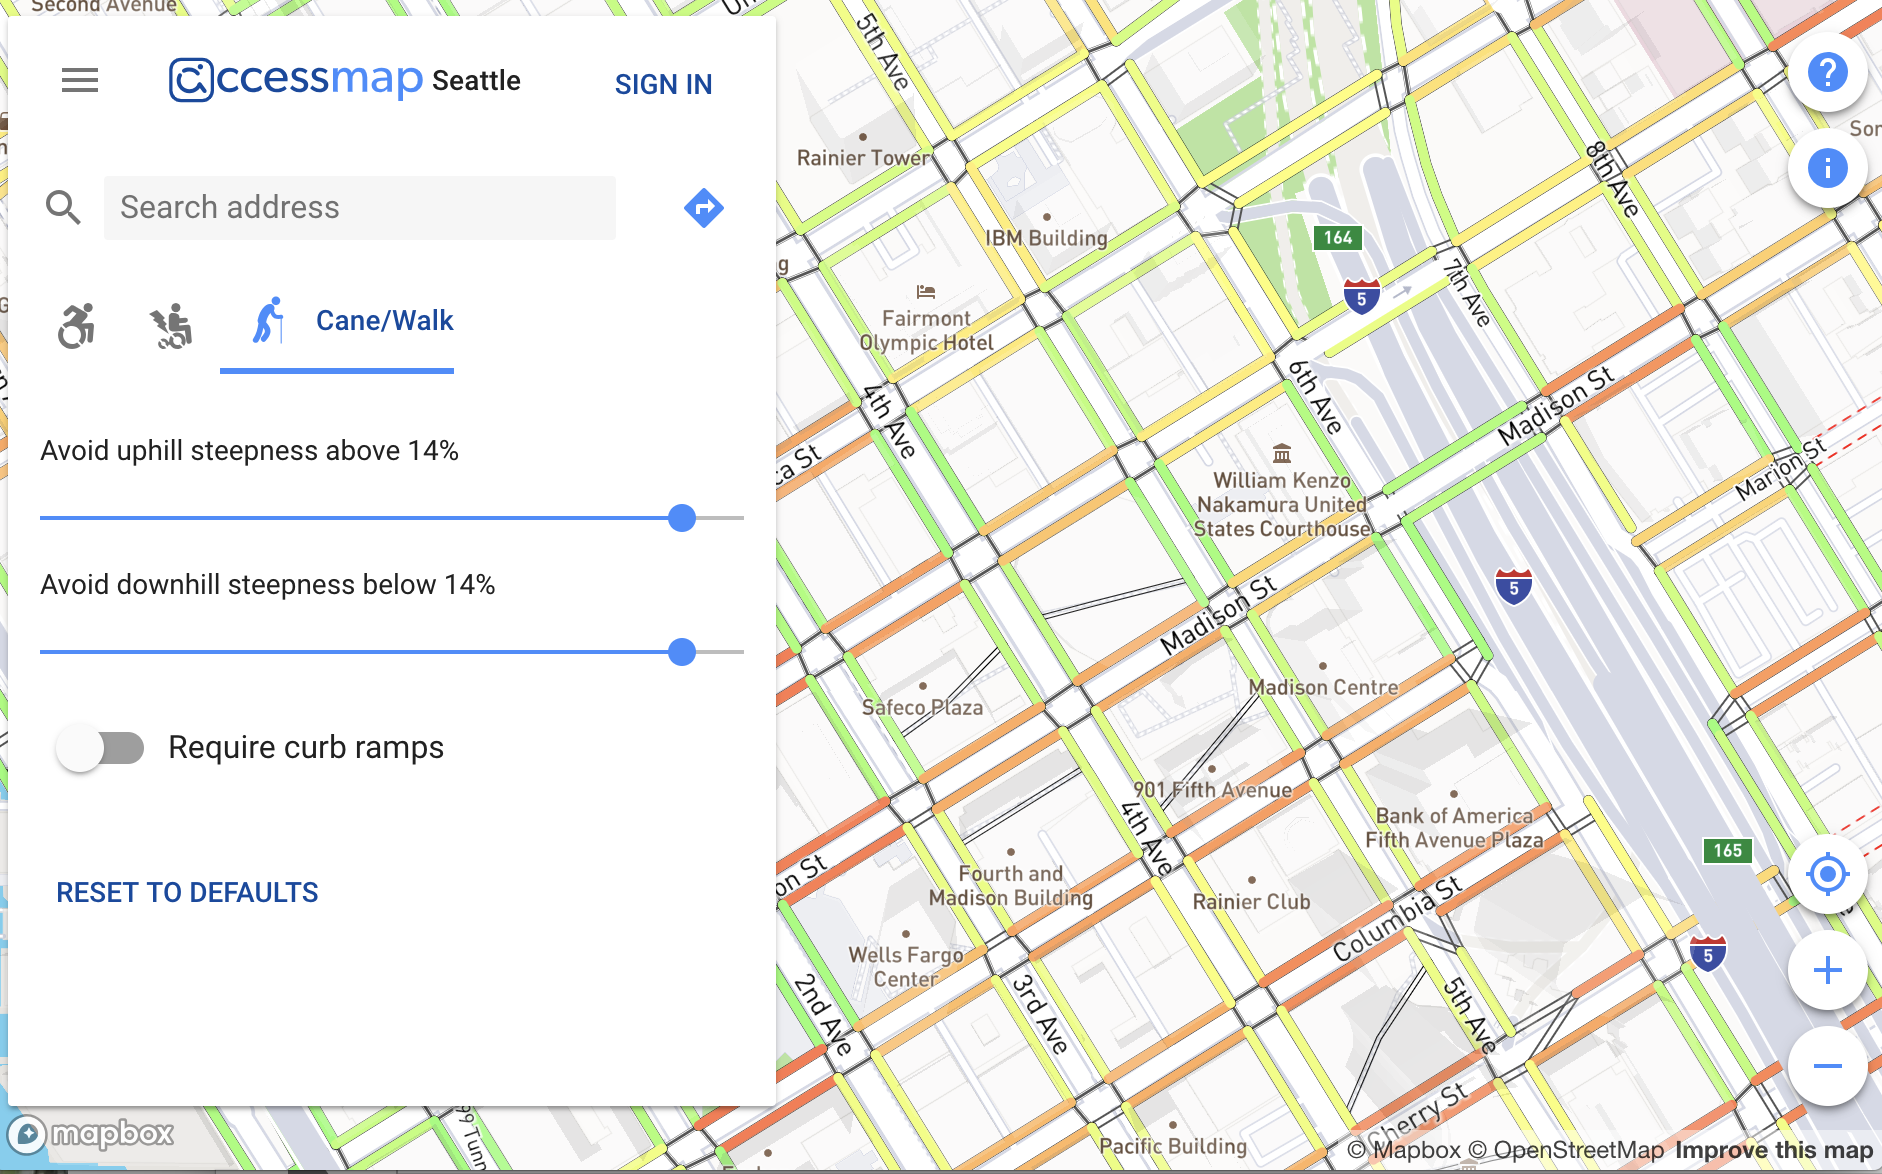
\includegraphics[width=5in]{pics/accessmap.png}
    \caption{AccessMap Screen Shot}
    \label{fig:accessmap}
\end{figure}

AccessMap currently can produce parametrically designed maps that always show the most up to data open data (derived from OpenSidewalks) about a region. 

\subsubsection{Proposed Development}

Operating hand-in-hand with AccessMap and OpenSidewalks (two projects discussed below), the goal of our work is to extend AccessMap to support users to automatically generate a custom 3D map model of any given area.  That model could then be printed at home, brought to a local library, or sent to a 3D printing service for relatively quick and inexpensive map production.  Beyond customizable map locations, ultimately the application would allow users to specify different scales and map features that are important to them.  

We will base our tactile design features on the comprehensive set of tactile map graphic symbols adopted by Braille Authority of North America (BANA) as created by (\cite{lobben2012tactile}, p. 107).% integrated into data driven design development tools and made available and consumable to landscape architects

%Anat: I commented this text out because I don't think it is product focused enough for NIDILLR's FIP in development. 
%The Tactile Maptile project designed the set of associated atomic symbols for that critical information.  Not only does this have implications for the map tiles specific to this project, but also more broadly works towards elevating pedestrian infrastructures in the context of our digital landscape.  This is important from a navigational perspective, but is also a reflection of the information designers, planners, and policy makers depend on to make significant decisions that affect our urban fabric.  Informed decisions based on incomplete data are not only difficult but also more prone to error and bias.  As we move rapidly towards sensor laced smart cities, it is critical these gaps be identified and understood in order to account for this influence on design and decision-making.  As such, this work is meant to take an accessible approach to data as it relates to pedestrian design and experience.

%Illustrative documentation of both the process and analysis that went into making these maps is directed more squarely at the design community. This project re-examines the pedestrian environment, with a focus on the specific needs of the low vision and blind communities. The goal of this work is to persuade designers to consider a broader spectrum of experience, and engage more critically in what it means to be designing inclusive cities.  

%This project is meant to bring attention to the deficiencies of the system currently place, in which accessibility checklists too often are accepted in lieu of truly inclusive design.  The straightforward approach is intended to remind designers that accessible design is good design, and if we want to build more equitable cities that means there is a huge spectrum of experiences we must first understand. 

\subsubsection{Validation}

\jm{ All studies need the following subsections to conform to the RFP:
\paragraph{Sample}
\paragraph{Environment}
\paragraph{Test Trials}
}

\ac{ needs writing


Our solution combines simple accessible interfaces with complex data integration and smart routing. To our users, the entire solution will be seamlessly presented in a workflow through which the travelers access a website, select the area of travel, the type of travel they wish to undertake in the area and travel preferences. The travelers are given the opportunity to verify the map location and features \textit{via} non-visual text-based exchange before printing the map.
% means what? A: means that in our UI pilot we found one of hardest things with building this UX/UI is ensuring that the tactile map model they got isn't of [Paris, Texas] when they actually meant [Paris, France]

The entire exchange is enabled and specifically designed for a portable 14-cell Braille-display. At the end, the traveler receives access to a downloadable 3D model file, access to an online URL where the model can be accessed for a specified duration, the option to have the model printed and sent to the user for a fee, and the option to subscribe to email alerts regarding any changes to the mapped region in the digital map repositories. 

}


\subsection{Automatically optimize map design based on specific needs (Mankoff\&Caspi-optimization.tex)}

\subsubsection{Background and State of the Art}

Route planning requires information that may be specific to the person creating a map. For example, Google Maps routes pedestrian directions from University Street Station on Second Avenue to Seattle City Hall on Fifth Avenue up Seneca Street, which has a steep 10 percent grade that is problematic for people in wheelchairs or with certain injuries or health conditions.
%SK:  how about older people?  That's not a "health condition" to me :).
%In contrast, AccessMap routes people two blocks north to Pike Street, which has a much gentler grade of less than 2 percent.
%For such people, it is important to ensure that a map clearly indicates slope. For those concerned about safety, however, it might be more important to show whether a guard rail is present near a particularly busy street, whether a sidewalk is wide or narrow near a busy street, or whether an alternative pedestrian route connects their sidewalk to a pedestrian footpath removed from the road. 
%For accessibility, 
users have varied needs.  A powered wheelchair user may need to know the location of curb ramps to navigate an intersection. A blind user may want to actively avoid certain types of curb ramps (such as those pointing to the center of an intersection). These different informational requirements present a particularly difficult situation to resolve without a detailed description of the available paths, how they are connected, and particular attributes (like curb ramps and their locations) \cite{bolten2017}. Furthermore, it is not possible to represent every possible piece of important information on any map. In particular, the amount of information that can be represented is further reduced in a tactile map. 
%SK:  Explain reason for preceding statement.

%SK.  Start discussion here.
\textit{Optimization} algorithms makes tactile maps accessible and actionable.  Here, we describe both: (1) optimizations that balance information richness with tactile usability, and (2) optimization cost functions that allow customization by Deaf-blind users of varied aspects of their travel experience.
%SK:  Now define optimization and what it does.

\jm{does this go in introduction instead?. also more about what optimization is/does A: I think that's where we were going before and it blew up the introduction. I think it's important to highlight here how optimization can make these maps actionable.}

\subsubsection{Previous Development: Optimization Approach}
Maps use many renditions to represent various forms of information. A  rendition could be a type of icon, or a colored line. Each rendition can represent only one class of information in a map. For example, a circular icon could note an accessible intersection, or a guide-dog friendly coffee shop, but it would be confusing if it represented both. Not all forms of information are compatible with all renditions. You cannot represent a road with just a circular icon. 
%The binary value stating if a a piece of information (a.k.a., a datum), $d$, is compatible with an rendition, $r$, is denoted $c_{rd} \in \{0,1\}$. If the datum is then assigned to a compatible rendition, this is denoted with the binary value: $x_{rd}\in \{0,1\}$

Our goal is to assign the most relevant pieces of information to the most useful renditions while maximizing the amount of information we present.  To do this, we need a model that describes what the most relevant information is.

%The zero-one linear program is formulated as follows:
%\begin{equation*}
%\textrm{ argMax }
%\sum_{i=1}^{|R|}
%\sum_{j=1}^{|D|}
%\alpha(r_i, d_j) x_{ij}
%\end{equation*}

%\begin{subnumcases}{
%\textrm{ s.t. } 
%}
%   \forall_{i \leq |R|} \forall_{j \leq |D|} r_{ij} x_{ij} \leq r_{ij} \label{data_rendition_compatability}\\
%   \forall_{i\leq|R|} \sum_{j\leq|D|} x_{ij} = 1 \label{rendition_Cap} \\
%\forall_{j\leq|D|} \sum_{i\leq|R|} x_{ij} \leq 1  \label{unary_data}\\
%\sum_{i\leq|R|} \sum_{j\leq|D|} x_{ij} = %\min(|R|, |D|) \label{complete_fill}
%\end{subnumcases}

%\item[Weighting Information-Rendition Pairings]
Specifically, when deciding how (or whether) to render a piece of information, we must consider three features with the acronym (CIA): the rendition's communicative ability (C), the data's importance (I), and the attentive cost (A).
%SK: Will readers know what "attentive cost" means? You use this interchangeably with "attention cost."  I changed all refs to the former for consistency.
We combine these by subtracting the attentive cost ($A$)  from the benefits ($C*I$): 
\begin{equation}
\label{eq::CIA}
\alpha(r_i, d_j) = C(r_i, d_j)*I(d_j)-A(r_i, d_j)
\end{equation}

\begin{description}
\item[Communicative Ability]
Communicative Ability, $C(r,d)$, is the measure of how well a rendition, $r$, communicates a specific type of information, $d$.
%A high level measure of this is already accounted for in the hard constraints of the linear program: if a rendition is incompatible (\ie incapable of communicating a class of information) constraint \ref{data_rendition_compatability} will not be met and the pairing will not be accepted. But our model must support more nuanced expressions of information communication. 
%For instance, there may be many types of renditions that label a coordinate on a map, but each are subject to certain limitations. 
For example, the number of parallel roads that can be represented in a space depends on the width of the lines representing the roads; denser road networks require thinner lines, while sparse networks could make use of more distinguishable, thicker lines. Further, certain attributes of a rendition may be more or less desirable to a specific user, such as the preference for braille or embossed text. 
%In our system, all renditions have a set of attributes, $a \in A_r$, (\eg uses braille, uses raised edges vs uses indented edges). Similarly, users profiles, $U$, and classes of information, $d$, have a set of preferred attributes, $\hat{A}_U,\hat{A}_d$ and weights on those preferred attributes $\beta_a$. 
More formally, the communicative ability of an information-rendition pairing is the weighted sum of the intersection of a rendition's attributes, an information class's preferred attributes, and a user's preferred attributes. 
\begin{equation}
\label{eq::communicability}
C(r,d,U) = \sum_{a\in A_r \cap \hat{A}_d}(\beta_a) +  \sum _{a\in A_r \cap \hat{A}_U}(\beta_a)
\end{equation}
%Attributes can be expressed in many ways, and determining the intersection of a rendition's attributes and preferred attributes is managed through a series of adapter interfaces. For instance, one interface is a Braille-compliant rendition, which requires the rendition to generate related text in braille. A user profile and information maintains a list of relevant adapters (\ie the preferred attributes) mapped to the preferential weight and any parameters of that preference. An example parameter is a preference for lines no thicker than 2 mm or no shorter than 1mm. These parameters are applied to the rendition through the adapter. 

\item[Information Importance]
%Information importance is the simplest measure of an Information-Rendition Pairing and it is central to the adaptive design paradigm our system represents. 
Users know what information is important to them. They know the accessibility features and challenges that affect them most, and what points of interest are most relevant to them. %For this measure, we simply 
Thus, we ask users to rank information. %, the higher the ranking, $I(d_j)$, of a class of information, the higher the weight. If the information is useless or irrelevant to the user the ranking is set to zero which intern makes the weight, $\alpha$, on all rendition pairings with this information zero or less, guaranteeing that the information will not be presented. For efficiency reasons, information classes that are marked as having no importance are excluded from linear program a priori. 
We can pre-populate this with default rankings based on a survey of typical user preferences. 

\item[Attentive Cost]
The attentive cost of a rendition measures how distracting it is to gather information from it. For example, if a user were using a rendition of a road network to navigate the map in search of a target, say their favorite coffee shop,  the longer it takes to find the target the more information they must keep track of (\textit{e.g.,} where they started, what turns they made, what landmarks they noticed). Tracking all of this information carries an attentive cost that would otherwise be spent on the primary search task.

A key problem here is that when the map is being constructed and the attentive cost weight is needed, we do not know what the user's target(s) will be, where they will start their search, or what other information is presented that may help or hinder the search task. To address this, we will use a Monte-Carlo simulation of user behavior based on our experimental work.\jm{megan: reference for monte carlo?} %The presentation of that information is, in fact, our goal. Given this level of uncertainty, we use a Monte-Carlo simulation to estimate the average \textit{time} it takes for the user to perform a search given a rendition-information pairing. The probability distribution used to generate this Monte-Carlo simulation is derived from a Markov-chain state model representing the actions a user can take when he or she encounters portions of a rendition. 
%\begin{figure}
%\label{fig::exampleStates}%
%	\begin{tikzpicture}
%        % Add the states
%        \node[state] at (0, 0) (o) {Off Road};
%        \node[state] at (4, 0) (r) {On Road};
%        \node[state] at (2, 4) (i) {Intersection};

%        \draw[every loop]
 %       	(i) edge[loop left] node {} (i)
%        	(i) edge[bend right=20] node %{} (r)
%            (r) edge[bend right=20] node {} (i)
%            (i) edge[bend right=20] node {} (o)
%            (o) edge[bend right=20] node {} (i)
%            (o) edge[loop left] node {} (o)
%            (r) edge[bend right=20] node {} (o)
%            (o) edge[bend right=20] node {} (r)
%            (r) edge[loop right=20] node {} (r);
%    \end{tikzpicture}
%\caption{Example of states of navigating a road network}
%\end{figure}
\end{description}

%Suppose that a user is navigating a rendition of a road network. There are three basic states of the action: (1) moving a finger along the road, (2) encountering an intersection of roads, and (3) moving a finger along the new road. Which particular state the user is in depends on the specific roads paired to the rendition, and their likelihood of moving from one state to another depends on both the particular road network (the information) and the rendition. For example, when the user encounters an intersection, he or she is very likely to continue onto a new road (\eg changing from the Intersection to On-Road state), but which road depends on many factors. Generally, the user is more likely to move in the same direction and increasingly less likely to turn all the way around. If the rendition presents very thin roads, the user is more likely to travel in a direction that they don't feel the roads any more, moving into the "Off-Road" state. We model the probability of this state change by selecting a random angle between $-\pi$ and $\pi$ from a normal distribution with a mean direction of 0 (no change in direction from the approaching road). If the user travels in that direction but could still feel a road (based on the width of the finger and thickness of the rendition), then the angle will be modified to continue along that road, otherwise they will move randomly in that general direction off-road until they find a new road to follow.  

%Each state change in the Markov-chain takes about step of one finger width, and we use a state change as a unit of time. For each simulation in the Monte-Carlo model, the user takes a "walk" across the map starting at a random point and moving towards a target. The starting points and targets are selected from a probability distribution where areas denser with information are more likely to be selected. The Markov-chain determines the walk that they take. We count the number of steps in the walk it takes to find the target given the rendition and information. The average number of steps over many models is our attention cost, meaning the more difficult (the longer it takes) it is to find information using a rendition-information pairing, the greater the attention cost and the poorer the pairing. 

%In terms of implementation, each rendition, $R$, has a set of states $S_R$. The probability of entering a state, $s_i\in S_R$, is dependent on the data, $D$, paired to $R$ and the state it is entering from, $s_{i-1}$: $P(s_i | D, s_{i-1})$, A walk over the map, $W$, starts from a starting point/state $s_1$ and we randomly change the state based on the probability distribution of all possible next-states. With each state we move the finger, $f$, a one finger width, $w_f$ in the direction dictated by the current state. The attention cost of a walk, $A(W)$, is the number of states need to get the point $f$ within $w_f$ of the target point $t$.The attention cost of a pairing, $A(R,D)$ is equal to the average attention cost of all of $N$ simulated walks.

%\begin{equation}
%W \subset S_R | s_1...s_{|W|}
%\end{equation}
%\begin{equation}
%A(W) = |W|
%\end{equation}
%\begin{equation}
%A(R,D) = \frac{\sum_{i=1...N} A(W_i)}{N}
%\end{equation}

\subsubsection{Proposed Development}

An optimization algorithm can use this information to decide on the optimal map. In optimization terms, $C*I-A$ is an \textit{objective function}, which can calculate a score for a possible map. Off-the-shelf algorithms can solve for the best solution (map in our case). For this problem, we can then  formulate the optimization as a zero-one linear program interpretation based on the Generalized Assignment Problem
\cite{kuhn1955hungarian}. 

\subsubsection{Validation}
\ac{JM: need your input here}
\ac{ make sure to include tests for both adequate balance for legibility and feature richness as well as tests for parametrization }

The following validation statements should be tested and hold true if the design goal for this development activity is met: 

The resulting tangible map depictions and choices will be valid.

\ac{this is just an example of a usability validation:}
When routing and choosing map features for no-vision pedestrians, the optimization algorithm favors streets with sidewalks and lower environmental stress (e.g., lower speed limits and traffic volume).

Here we describe our validation tests for both statements. The data elements and sources are referencing tests and data collection that will occur with our community partners. These data collection activities are described in later sections with greater detail.

\textbf{Validation Statement 1:
The resulting tangible map depictions and choices will be valid.}

\texttt{Performance Metrics:} 

\texttt{Data Elements \& Sources:}

\texttt{Analysis Procedure:}

\textbf{Validation Statement 2:
When routing and choosing map features for no-vision pedestrians, the optimization algorithm favors streets with sidewalks and lower environmental stress (e.g., lower speed limits and traffic volume).
}


\texttt{Performance Metrics:} 

\texttt{Data Elements \& Sources:}

\texttt{Analysis Procedure:}


\subsection{Validation: Iterative Design of Mapping Solution}

Describe tests trials and other related activities, and justify the choice of sample and environment. 

We will take a user-centered, iterative approach to the design of our mapping solution. All of our studies will be conducted with the population we are serving, Deaf-blind users. PI Caspi has extensive experience working with this population \jm{true?} and will be able to help ensure that we have access to participants. 

\subsubsection{Map Study 1: Map Understanding With and Without Optimization}
\label{sec:lab-tests}
Our first study will focus on demonstrating the benefits of optimization in a controlled fashion. For this study, we will use pre-defined maps focusing on neighborhoods familiar to participants. we will ask participants to indicate the location of a well known landmark, and to describe the region around the landmark. We will also ask participants to describe features of a route between two landmarks. We will then have them do the same tasks with an optimized map. \jm{how do we ensure famimliarity? do we care about route finding? How do we make sure the optimization is relevant to them? How do we train them on all the renditions' meanings?+}

\subsubsection{Technical Validation}
\sec{sec:technical-validation}

\subsubsection{Map Study 2: Navigation Benefits of Optimization}
\label{sec:field-map}
\jm{I think we also want a study of them choosing a route of their choice and using our system?}

\subsubsection{Map Study 3: End-to-end system use}
\label{sec:field-web}
\jm{test that they can produce a map on their own when they want and use it}


\subsection{Input from Stakeholders}
Describe how input will be collected from key stakeholders (including people with disabilities) to guide development activities.

\subsection{Stage of Development and Specific Plan}

This project includes both the \textit{proof of concept} stage and the \textit{proof of product} stage:
\begin{description}
\item[Implementing and Testing Optimization Algorithm (Proof of Concept)] While we have preliminary results demonstrating the viability of optimization for this problems space \ref{sec:optimization}, our proposed work includes recruiting and testing with Deaf-blind individuals \ref{sec:lab-tests}, and resolving remaining challenges in optimization \ref{sec:optimization}.
\item[Testing in Natural Contexts (Proof of product)] Our proposed work also includes field studies. We will be testing the map in use in field settings \ref{sec:field-map}, and testing the entire system (including web-based map creation) in the field \ref{sec:field-web}. 
\item[Fully Integrated Prototype (Proof of product)]
Our final implementation will be integrated into AccessMaps, a publicly available mapping application. \ref{sec:accessmaps-integration}.
\item[Verification of Technical Requirements (Proof of product)]
We will validate the generalizability of our approach \jm{keep this? What is the appropriate technical validation?} \ref{sec:technical-validation}
\end{description}
    

\subsection{Enabling User to Produce Maps Themselves (Mankoff)}


\subsection{Conclusion}
needed?